\documentclass[journal]{IEEEtran}

\renewcommand\thesection{\arabic{section}} 
\renewcommand\thesubsectiondis{\thesection.\arabic{subsection}}
\renewcommand\thesubsubsectiondis{\thesubsectiondis.\alph{subsubsection}}
\renewcommand\theparagraphdis{\arabic{paragraph}.}

%\usepackage[retainorgcmds]{IEEEtrantools}
%\usepackage{bibentry}  
\usepackage{xcolor,soul,framed} %,caption

\colorlet{shadecolor}{yellow}
% \usepackage{color,soul}
\usepackage[pdftex]{graphicx}
\graphicspath{{../pdf/}{../jpeg/}}
\DeclareGraphicsExtensions{.pdf,.jpeg,.png}

\usepackage[cmex10]{amsmath}
%Mathabx do not work on ScribTex => Removed
%\usepackage{mathabx}
\usepackage{array}
\usepackage{mdwmath}
\usepackage{mdwtab}
\usepackage{eqparbox}
\usepackage{url}
\hyphenation{op-tical net-works semi-conduc-tor}
\usepackage{graphicx}
\usepackage[T1]{fontenc}
\usepackage{dblfloatfix}    % To enable figures at the bottom of page




%\bstctlcite{IEEE:BSTcontrol}
%=== TITLE & AUTHORS ====================================================================
\begin{document}

\bstctlcite{IEEEexample:BSTcontrol}
    \title{
    	
\includegraphics[width=5in]{../imgs/logo_paper3.pdf} 
    	\newline
     Identifying a Trial Population for Clinical Studies on Diabetes Drug Testing with Neural Networks \\ 
     }

  \author{\textbf{L\"OHR Tim} \\ Friedrich Alexander University \\ \textit{tim.loehr@fau.de}}


% The paper headers
\markboth{Final Paper for the Machine Learning in the Industry 4.0 Seminar at the Machine Learning and Data Analytics Lab at the FAU 
}{Roberg \MakeLowercase{\textit{et al.}}}


% ====================================================================
\maketitle
% === ABSTRACT 
\begin{abstract}
%\boldmath
This project aims to model an end-to-end workflow of implementing Artificial Intelligence (AI) for the clinical environment. A possible use-case such as the selection of patients for a novel treatment or drug will be conducted by estimating the hospitalization time with a Neural Network.
The diabetes readmission dataset from the University of California, Irvine (UCI) Diabetes was used for this project. The trial population is selected by predicting the expected days for a person being hospitalized. Then and arbitrary boundary is set for chosing whether or not this patient is shall be included or not. If so, a clear explanation of the how the prediction was calculated and additional possible risk factors will be given in order to make the workflow explainable. This project shows that given a proper explanatory approach, AI can be a useful tool for the modern clinical environment. The workflow finally reveals that AI can be a beneficial support tool for doctors, e.g. by effectively choose possibly suitable patients in the patient selection process. 
\end{abstract}

% === KEYWORDS 
\begin{IEEEkeywords}
\hl{Machine Learning in the Industry 4.0, Clinical EDA, Data Analysis, AI in Medicine, Neural Networks, Diabetes, FAU, Department of Computer Science}
\end{IEEEkeywords}

\IEEEpeerreviewmaketitle

% === I. Project background and motivation
\section{Introduction}
\IEEEPARstart{D}{}ue to the upcoming new law enforced by the German Health Minister \textit{Jens Spahn}, electronic patient files will be nationwide standardized in Germany \cite{spahn} on the first of January 2021. This opportunity can be used to increase the impact of artificial intelligence on the health system to improve the health of Germany's population and facilitate doctor's work. Electronic health records (EHR) offer a variety of different application fields \cite{cite1} \cite{cite2}, such as: \\

\begin{itemize}
	\item Discover novel disease treatments
	\item Improve patients diagnosis
	\item Improve personalized healthcare \\
\end{itemize}

As of today in 2020, there are 7 million cases of diabetes in Germany, stated from the Robert Koch Institut (RKI) \cite{diab}. Compared to Germany's population size of 83 million people, 7 million diabetes cases are a credible amount that needs to be taken care of. Even for well known deceases like diabetes, there is continuous research and novel drugs and treatments are invented on a frequent basis. Still, not every person is suitable for obtaining a novel treatment. 

The project's background is an artificial scenario. The assumption is that the data is derived from the database collected through the new central storage system of the patient files due to the new German law. The typical name for medical data collected from hospitals is Electronic Health Records (EHR) as already mentioned in the abstract. Those EHR are under high data privacy rights conditions. They could only be used, if the data is completely anonymized and patients can not be traced back. So the assumption takes care of this issue and it is pretended that all those limitations and regularities have been successfully acquired.

After preparing the EHR for this privacy requirements, the data can now be utilized to gain insights and evaluations out of it. To use AI in the real-world clinics is a highly classified realization, because wrong decisions can cause a dangerous outcome towards patients. For this reason, implementing AI in Medicine requires a very detailed explanatory analysis of the predicted outcome. Keeping the background in mind, this project now aims to implement an end-to-end workflow of how to make use of AI in the real clinical environment. 

The first step is to figure out which patients are most likely suitable for receiving novel diabetes treatments. This can be achieved by a patient selection process, as stated by Dr. Toddenroth et. al. from the FAU \cite{cite4} and a more recent paper from Szu-Yeu Hu et. al. \cite{cite3}. Then the uncertainty estimation of the prediction is computed with the Aequitas tool from the University of Chicago. This estimation is performed to explain with Explainable Artificial Intelligence (XAI) methods how the prediction was determined. That process is supposed to enable an understanding of how certain estimations of Neural Networks are with respect to different dataset balance problems, e.g. demography. The research question for this project can therefore be concluded as: \\

\textit{Can Machine Learning be safely applied in the real clinical environment if it just provides enough explainability for its predictions?} 

% === II. Procedural Method==================================== 
\section{Methods}
\begin{figure}
	\centering
	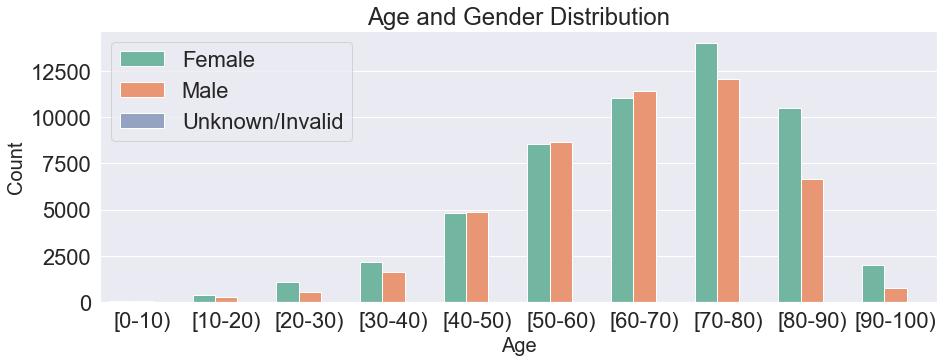
\includegraphics[width=1\linewidth]{../imgs/age_new}
	\caption{Age and Gender Disparity within the dataset}
	\label{fig:age}
\end{figure}

\begin{figure}
	\centering
	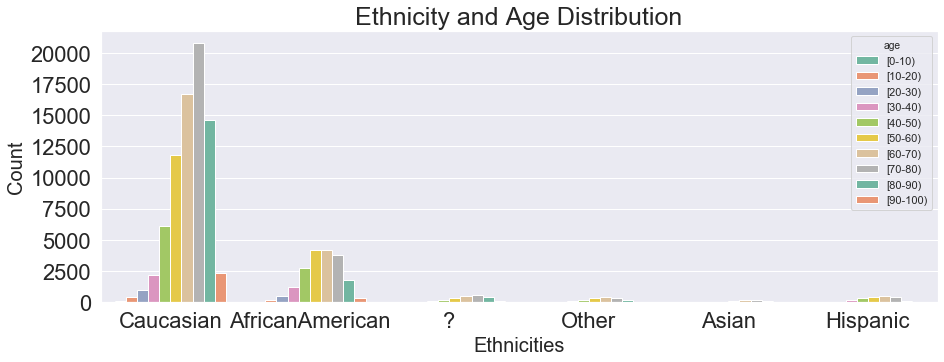
\includegraphics[width=1\linewidth]{../imgs/ethnicities_new}
	\caption{Ethnicity Disparity within the dataset}
	\label{fig:eth}
\end{figure}

\noindent The dataset is originated from the UCI Machine Learning Repository \cite{uci} collected from 1999 to 2008 with over 100000 entries to train on. Various features such as demographics, diabetes conditions or medications are provided. In total there are 55 features from which 36 are included for the modeling, because the other 19 features where useless due of missing features and NaN values. An important detail is the distribution of ethnicity, gender and age. This disparity is used in section results for evaluating the uncertainty of the model. Figure \ref{fig:age} and \ref{fig:eth} show that the median age of diabetes patients is around 70 to 80 years. The gender can be mostly ignored, because it is almost equally distributed among all patients. The ethnicity disparity reveals the biggest concern, because among different ethnicities there is a huge distribution gap. Asians and Hispanics are very underrepresented and African American people in comparison to Caucasian people as well. This plays an important role in the later predictive analysis and explanatory approach. Keeping these distributions in mind, the methods used for this project will be conducted in the following respective order: \\

\begin{itemize}
	\item Model a Neural Network 
	\item Explain the model with Uncertainty Estimation and Metrics (\textbf{why} are the model's predictions good)
	\item Explain the predictions with SHAP and LIME \\ (\textbf{how} is the prediction computed) \\
\end{itemize}

SHAP is a python package for approximating the so-called Shapely values. Those values can be used for various explanatory approaches, but for this project it is used for plots only like in Figure 7. LIME is a python package used for the lime XAI approach. Further explanations of those two approaches would exceed the limits of this report.
	
Preprocessing is most of the time the first step before modeling a Neural Network. Various unnecessary features were needed to be eliminated and categorical features were transformed into a one-hot encoded representation in order to funnel them into the Network properly. A supervised Neural Networks always has a response variable, a so-called label, in order to make a proper prediction by calculation the loss and doing backpropagation. The \textit{time in hospitalization} feature is used for this purpose, because it reveals the severity of each patient's diabetes decease. Usually, the longer people need to be hospitalized after receiving treatments, the worse the condition of the person is. So predicting a low hospitalization time with a novel treatment can indicate compatibility with the patient and so he or she is a good match to be selected. 

Neural Networks are able to achieve far better results than standard Machine Learning approaches like the Logistic Regression, due to the universal approximation theorem, yet they are less explainable. The Neural Network is modeled with a Keras sequential Neural Network, consisting of Dense, Dropout, Dense Variational and a Distribution Lambda layers to estimate the hospitalization time with a certain probability. The Distribution Lambda layer from Tensorflow incorporates an ensemble of models which report the variability of the prediction. It can be viewed as taking the mean of various regressions and measure the qualitative difference between all outputs. Those layers are implemented to eliminate the risk of: \\

\begin{itemize}
	\item Aleatoric Uncertainty: statisical uncertainty (\textit{known unknowns})
	\item Epistemic Uncertainty systematic uncertainty (\textit{unknown unknowns})\\
\end{itemize}

which usually occurs in clinical data. The aleatoric uncertainty will be evaluated with respect to the ethnicity distribution of the data. The epistemic uncertainty would break the limits of this project.

The neural network's prediction will be measured based on different evaluation metrics: \\

\begin{itemize}
	\item Precision, Recall and F1 Score
	\item Brier Score
	\item AUC Score \\
\end{itemize}

The loss function for the backpropagation is the negativ log likelihood function: 

\begin{center}
	Loss = \(-log(y)\) for each prediction \(y\) \\
\end{center}

The loss generally increases when the regression is unclear and shrinks with more certainty. At this point, the model is able to predict how long a person is going to stay in the hospital with respect to the demographics. The loss has a direct influence on the performance of the metrics. Generally speaking, if the loss is zero, all the metrics are supposed to have a perfect score.

Conclusively to guarantee full transparency of the patient selection process, Shapely values and LIME try to explain which features led to which output. In other words, which features have a positive and a negative impact on the hospitalization time. The key difference between those two XAI methods is that Shapely values want to explain \textit{how} one feature contribute to the overall prediction, while leaving out other combinations of features. LIME wants to explain what the most important features were for the prediction in general.

\begin{figure}[!b]
	\centering
	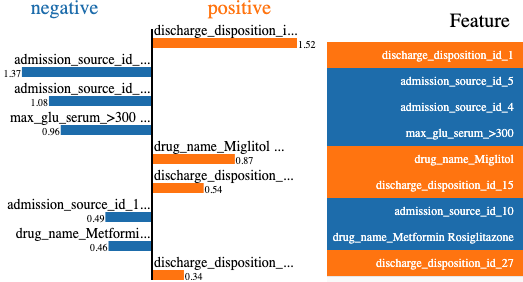
\includegraphics[width=1\linewidth]{../imgs/lime_paper}
	\caption{Important features computed by LIME. The true label for this was 7 days and model predicted a value of 6.42 days.}
	\label{fig:lime}
\end{figure}


%
%==================================================
%
\section{Results} 
\begin{figure}
	\centering
	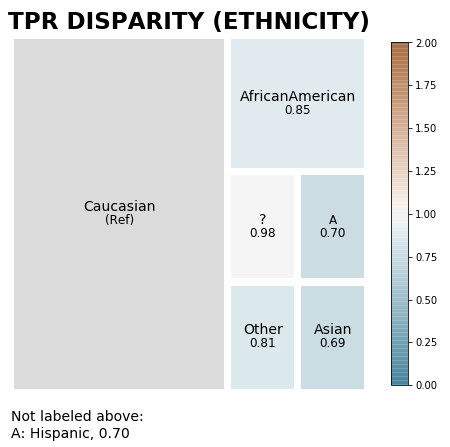
\includegraphics[width=0.8\linewidth]{../imgs/tpr_paper}
	\caption{True positive rate among ethnicities with Caucasiens as reference group with the discrimination boundary at day four}
	\label{fig:tpr}
\end{figure}

\begin{figure}
	\centering
	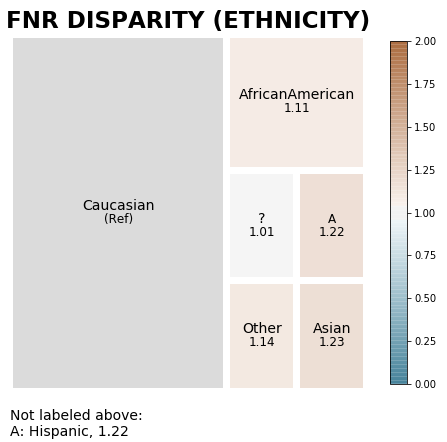
\includegraphics[width=0.8\linewidth]{../imgs/fnr_paper}
	\caption{False negative rate among ethnicities with Caucasiens as reference group with the discrimination boundary at day four}
	\label{fig:fpr}
\end{figure}

\begin{figure*}[!b]
	\centering
	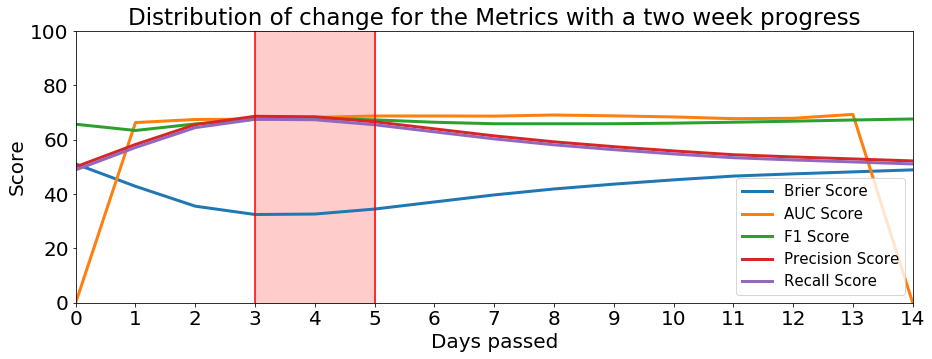
\includegraphics[width=0.9\linewidth]{../imgs/metrics_time}
	\caption{The graphic shows the temporal change of the metrics with respect to a different time constraints on the boundary. The best values for the metrics can be found between the third and fifth day. Setting the boundary somewhere in the red highlighted area produces the best and most certain estimation.}
	\label{fig:change}
\end{figure*}


\noindent After having the workflow in mind, the first step is to train the neural network and evaluate its results. The model trained for 50 epochs and reached a loss of 2.97. Figure \ref{fig:change} shows the course of events for different evaluation metrics. For example, the \textit{Brier Score} itself is best when it is as low as possible. The other scores are best, when they are as close to 100 percent as possible. The X-Axis represents the predicted time of hospitalizations in the unit of measurement days. All metrics have a optimal score for the boundary at day four, as can be seen in \ref{fig:change}. After selecting the most promising discrimination boundary at day four, the uncertainty estimation with respect to ethnicity can be computed. 

Figures \ref{fig:tpr} and \ref{fig:fpr} reveal that the true positive rate for Caucasian people is higher compared to the other ethnicities. Also, the false-negative rate of other ethnicities is higher compared to the reference Caucasian people.  

The next step is the investigation of how each prediction was computed and what the most important features were. As mentioned in the section methods, Shapely and LIME are used for this purpose. 

\begin{figure}
	\centering
	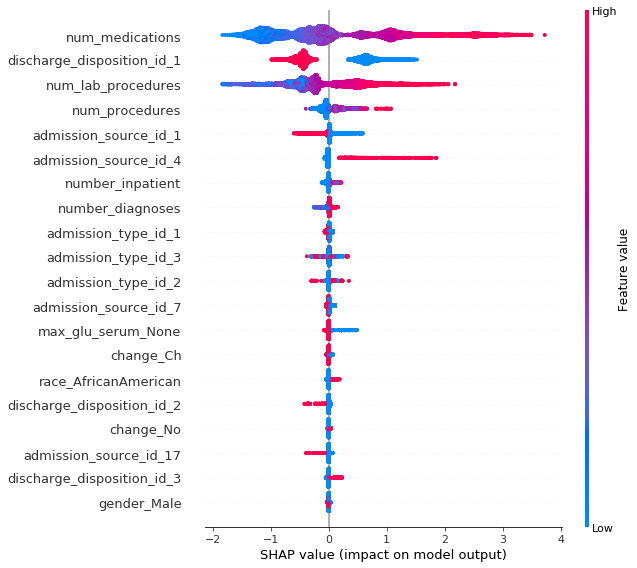
\includegraphics[width=1\linewidth]{../imgs/shap_paper}
	\caption{False negative rate among ethnicities with Caucasiens as reference group with the discrimination boundary at day four}
	\label{fig:shap}
\end{figure}

\begin{figure}
	\centering
	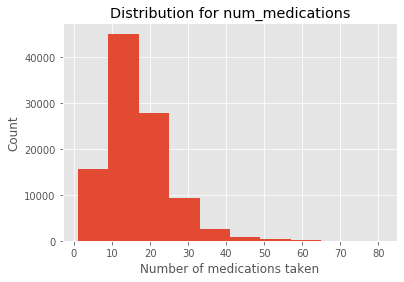
\includegraphics[width=0.9\linewidth]{../imgs/meds_dist}
	\caption{Normal right skewed distribution of the feature \textit{num\_medications}}
	\label{fig:num_meds}
\end{figure}

The second interpretational approach are the Shapely values, which can be seen in Figure \ref{fig:shap}. This figure lists 20 of the features with their both positive and negative on impact on the prediction of the hospitalization time. Negative values on the X-Axis have an decreasing impact on the hospitalization time and positive values on the X-Axis will increase the time of hospitalizations.

%
% === II. 4	Data description with visualization==========================
%
\section{Discussion}
Training the model alone can not qualify for selecting a patient into the trial population. There needs to be a specific boundary indicating after which time of hospitalization the diabetes is so serious, that this person can be taken into consideration for the trial, otherwise the selection process can not be accomplished. Figure \ref{fig:change} not only shows the course of events, but it also reveals that different boundaries for the X-Axis produce diverse scores. The optima is between day three and day five. 

The uncertainty estimation can be evaluated for different demographics against each other and with different boundaries set on Figure \ref{fig:change}. Figures \ref{fig:tpr} and \ref{fig:fpr} indicate, that if a patient is being selected and he or she is Caucasian, the probability of a positive or negative choice is more accurate compared to other ethnicities. Looking back at Figure \ref{fig:eth}, this important prediction disparity can be explained due to the huge difference in training data for all ethnicities.

Shapely values and LIME need to be interpreted in a different way than the metrics. Figure \ref{fig:lime} illustrates the single components which led to this prediction of 6.42 days. The meaning of these categorical features are provided by the following bullet points: \\

\begin{itemize}
	\item discharge\_disposition\_id\_1: Discharged to home
	\item admission\_source\_id\_5: Transfer from a Skilled Nursing Facility (SNF)
	\item admission\_source\_id\_4: Transfer from a hospital
	\item admission\_source\_id\_10: Transfer from critial access hospital \\
\end{itemize}

This specific patient is marked with the features \textit{admission\_type\_id\_1} and \text{discharge\_disposition\_id\_6}. This means that \textbf{not} having the features \text{admission\_source\_id\_5} and \text{6} has an actually \textbf{positive} (fewer days in hospital) impact on the hospitalization time, whereas when a patient has the \textit{discharge\_disposition\_id\_1}, this indicates a longer stay in the hospital. Also e.g. if the patient is taking the medication \textit{Migitol}, he or she generally will stay up to one day (0.87) longer in hospital than people who do not take this drug. Explanations like this can be conducted for all 36 trained on features for further investigation and new insights into which effects medications or treatments have.

The distribution of \textit{num\_medications} can be seen in Figure \ref{fig:num_meds}. This distribution reveals a right-skewed normal distribution. Based on that distribution, it becomes obvious that a normally distributed numerical feature can have both a negative and a positive impact on the prediction of the most important features computed by SHAP, as shown in Figure \ref{fig:shap}. The more medications a person takes, the worse the condition and the longer the hospital stay for this person is, and vice versa. Whereas the feature \textit{admission\_source\_id\_4}, if marked positive for a person, has always a high positive impact (higher hospitalization time) for the patient.  

After taking all evaluations and explanatory steps into consideration, can Neural Networks safely be applied in the Industry 4.0 and especially hospitals? Keeping the results in mind, it appears that AI has many good traits why it should be applied. In total, the pro's have a higher weight, because the con's will vanish the more it is applied and the more mature these technologies will become. \\ 

\textbf{Pros}: 

\begin{itemize}
	\item Support for doctor's decision
	\item Patient selection saves a lot of time
	\item New insights of treatment of medication effects into the patients medical condition
	\item Possible new insights \\
\end{itemize}

\textbf{Cons}: 

\begin{itemize}
	\item Unstructured data
	\item Uncertainty if it can be applied among different EHR and not only diabetes data
	\item The minimum necessary needed data amount for highly explainable predictions is unclear \\
\end{itemize}

These techniques can be a good decision-support technology for doctors. If there are for example 2000 patients stored in the hospital's database, this selection process can already shrink the number of people that could possibly be suitable for receiving the novel treatment. Doctors will make the final decision based on their experience, but they can end up saving a lot of time by looking at already 20 pre-selected patients instead of investigating 2000 patient files. So even if the prediction is not going to be selected, it has no dangerous impact for patients in general. Doctors should be taught to develop more trust into a well trained and good performing AI system, because it can be beneficial for everyone.

 
\section{Conclusion}
\noindent The conclusion of this entire workflow leads to three final questions to be answered. \\

\textit{Apply it without additional doctor’s approval?} \\

For sure not. What if only one person dies because of a false decision of the Neural Network's prediction? This is a hot topic and the law and regulatory clinical instances like the FDA in the United States or the Arzneimittelbehörde in Germany comes into force when implementing such technologies in the clinical environment. \\

\textit{Apply it as a support technology?} \\

Sure if a doctor validates the results, it can be used to support the clinical trials and save up a lot of time and identify new interesting insights. \\

\textit{Does a combination of metrics improve the overall explainability and how many metrics are enough?} \\ 

Using at first the F1-Score for evaluating the model's performance and then computing the uncertainty estimation with respect to critical features has an overall improvement. Furthermore it could be seen that many different approach reveal different insights of the prediction. It becomes clear that a good combination of metrics enhances the overall performance a lot.


\section{Future Work}
\noindent For future research those further improvements can also be made, such as: \\

\begin{itemize}
	\item Try different XAI methods or explain more features with different ways
	\item Try different Neural Networks or classifiers with GPU for higher accuracies
	\item Model also the Epistemic Uncertainty with different Neural Network Layers: tfp.layers.DenseVariational for a more robust Network
\end{itemize}


\section*{Acknowledgment}
\noindent Thanks a lot to Philipp Schlieper from the Machine Learning and Data Analytics Lab for a really good supervising through out my project. I can totally recommend this seminar.



% if have a single appendix:
%\appendix[Proof of the Zonklar Equations]
% or
%\appendix  % for no appendix heading
% do not use \section anymore after \appendix, only \section*
% is possibly needed

% use appendices with more than one appendix
% then use \section to start each appendix
% you must declare a \section before using any
% \subsection or using \label (\appendices by itself
% starts a section numbered zero.)
%

% ============================================
%\appendices
%\section{Proof of the First Zonklar Equation}
%Appendix one text goes here %\cite{Roberg2010}.

% you can choose not to have a title for an appendix
% if you want by leaving the argument blank
%\section{}
%Appendix two text goes here.


% use section* for acknowledgement
%\section*{Acknowledgment}


%The authors would like to thank D. Root for the loan of the SWAP. The SWAP that can ONLY be usefull in Boulder...


% Can use something like this to put references on a page
% by themselves when using endfloat and the captionsoff option.
\ifCLASSOPTIONcaptionsoff
  \newpage
\fi



% trigger a \newpage just before the given reference
% number - used to balance the columns on the last page
% adjust value as needed - may need to be readjusted if
% the document is modified later
%\IEEEtriggeratref{8}
% The "triggered" command can be changed if desired:
%\IEEEtriggercmd{\enlargethispage{-5in}}

% ====== REFERENCE SECTION

%\begin{thebibliography}{1}

% IEEEabrv,

\bibliographystyle{IEEEtran}
\bibliography{IEEEabrv,Bibliography}
%\end{thebibliography}
% biography section
% 
% If you have an EPS/PDF photo (graphicx package needed) extra braces are
% needed around the contents of the optional argument to biography to prevent
% the LaTeX parser from getting confused when it sees the complicated
% \includegraphics command within an optional argument. (You could create
% your own custom macro containing the \includegraphics command to make things
% simpler here.)
%\begin{biography}[{\includegraphics[width=1in,height=1.25in,clip,keepaspectratio]{mshell}}]{Michael Shell}
% or if you just want to reserve a space for a photo:

% ==== SWITCH OFF the BIO for submission
% ==== SWITCH OFF the BIO for submission


%% if you will not have a photo at all:
%\begin{IEEEbiographynophoto}{Ignacio Ramos}
%(S'12) received the B.S. degree in electrical engineering from the University of Illinois at Chicago in 2009, and is currently working toward the Ph.D. degree at the University of Colorado at Boulder. From 2009 to 2011, he was with the Power and Electronic Systems Department at Raytheon IDS, Sudbury, MA. His research interests include high-efficiency microwave power amplifiers, microwave DC/DC converters, radar systems, and wireless power transmission.
%\end{IEEEbiographynophoto}

%% insert where needed to balance the two columns on the last page with
%% biographies
%%\newpage

%\begin{IEEEbiographynophoto}{Jane Doe}
%Biography text here.
%\end{IEEEbiographynophoto}
% ==== SWITCH OFF the BIO for submission
% ==== SWITCH OFF the BIO for submission



% You can push biographies down or up by placing
% a \vfill before or after them. The appropriate
% use of \vfill depends on what kind of text is
% on the last page and whether or not the columns
% are being equalized.

\vfill

% Can be used to pull up biographies so that the bottom of the last one
% is flush with the other column.
%\enlargethispage{-5in}



% that's all folks
\end{document}